
In this section we do some further analysis on the data gathered from LJ. 

\subsubsection{Do attractive people group together?}\label{sec:att_dist}

In order to better understand attractive members, we studied how they are distributed in the community. Are they distributed uniformly or do they follow some patterns.  Specifically,  for each community $\Cc$, we computed the percentage of attractive friends of all members $v\in\Cc$, i.e., for each member $v$, we computed
\[
\frac{\sum\limits_{v'\in\partial v \cap \Cc } a_{v'}}{\partial v \cap \Cc }.
\]  
For each community, we divided these numbers into two separate sets for attractive and unattractive people, and computed the average of each set. The box plot in Fig. \ref{fig: perc att} summarizes the statistics of these averages computed for the communities under study. There is a clear difference between the percentage of attractive friends of attractive and unattractive people. Attractive people seem to have a much higher percentage of attractive friends. 
\begin{figure}
\begin{center}
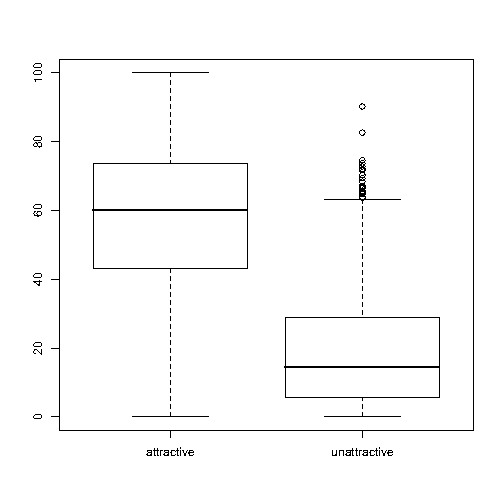
\includegraphics[width=80mm]{../figures/Rplot.pdf}\caption{Percentage of attractive friends of attractive/unattractive members}\label{fig: perc att}
\end{center}
\end{figure}

\subsubsection{Do social people group together?}

Similar to Section \ref{sec:att_dist}, we studied the distribution of social people in a community. For each person we computed the percentage of its friends that are social. Again we divided these numbers into two sets which corresponds to social and asocial people. Fig.~\ref{fig: perc social} summarizes the distribution of each set. It demonstrates significant distinction between the two distributions.  According to the plot, on average about $60\%$ of a social person's friends are social themselves, while this percentage is less that $20\%$ for an asocial person.
\begin{figure}
\begin{center}
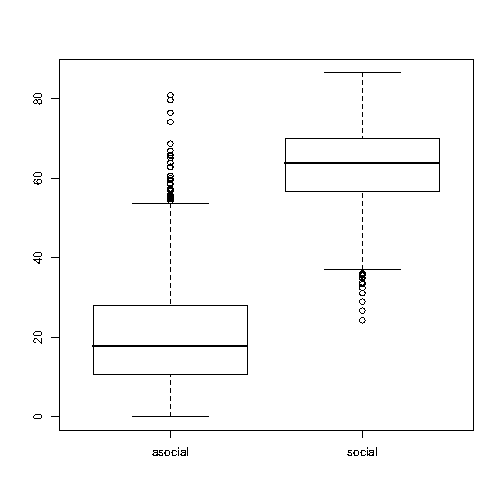
\includegraphics[width=80mm]{../figures/Rplot_soc.pdf}\caption{Percentage of social friends of social/asocial members}\label{fig: perc social}
\end{center}
\end{figure}


\subsubsection{Puzzle}

Several studies point out the fact that the growth of a community is highly dependent on its clustering coefficient.
This coefficient is defined as the ratio of closed to open triads in the friendship subgraph
induced by the members of a community.

\begin{figure}
  \begin{center}
    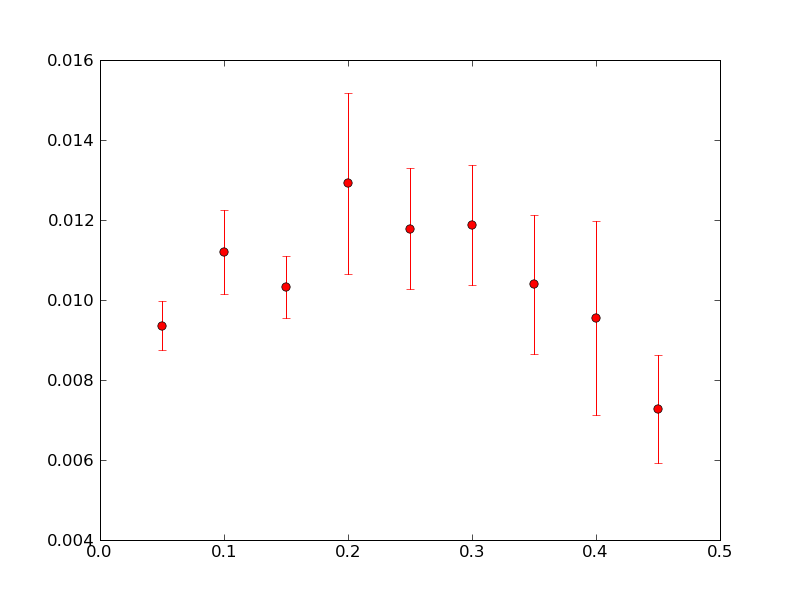
\includegraphics[width=8cm]{../figures/first.png}
    \caption{Community growth rates vs. ratio of closed to open triads: $1^{\rm st}$ snapshot}\label{fig:edge-a}
    \end{center}
\end{figure}

\begin{figure}
  \begin{center}
    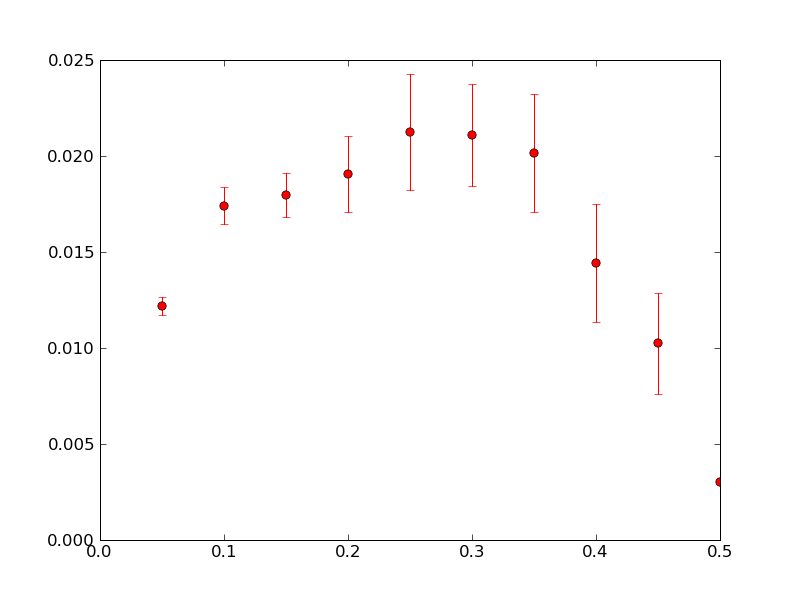
\includegraphics[width=8cm]{../figures/second.png}
    \caption{Community growth rates vs. ratio of closed to open triads: $2^{\rm nd}$ snapshot}\label{fig:edge-b}
    \end{center}
\end{figure}


\begin{figure}
  \begin{center}
    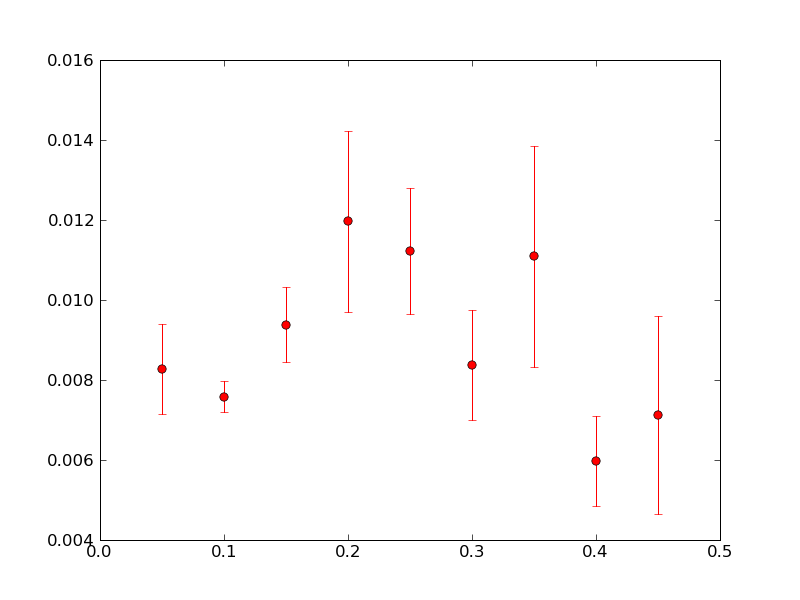
\includegraphics[width=8cm]{../figures/third.png}\label{fig:edge-c}
    \caption{Community growth rates vs. ratio of closed to open triads: $3^{\rm rd}$ snapshot}
    \end{center}
\end{figure}

\begin{figure}
  \begin{center}
    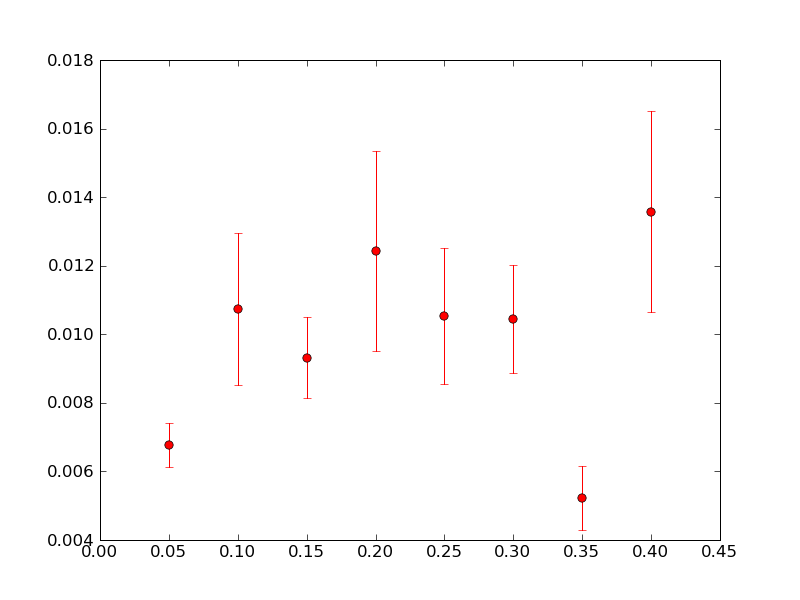
\includegraphics[width=8cm]{../figures/fourth.png}\label{fig:edge-d}
    \caption{Community growth rates vs. ratio of closed to open triads: $4^{\rm th}$ snapshot}
    \end{center}
\end{figure}

\begin{figure}
  \begin{center}
    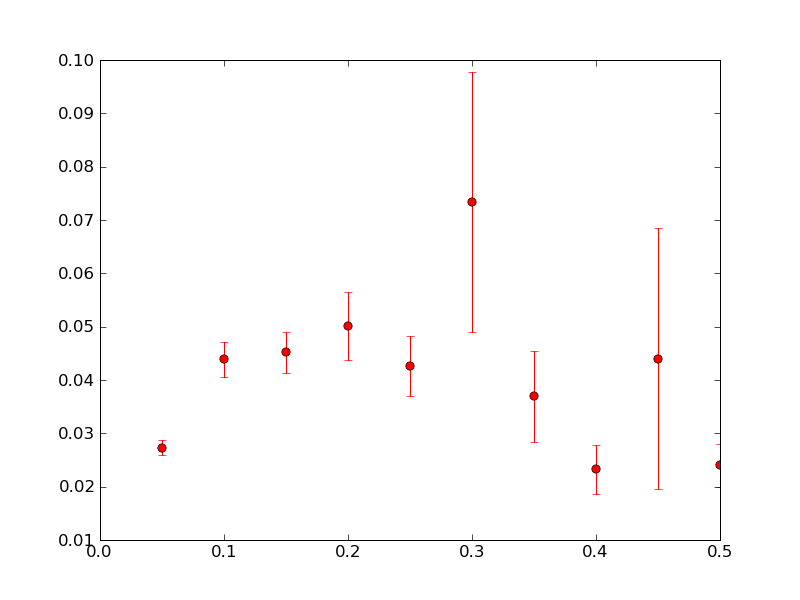
\includegraphics[width=8cm]{../figures/fifth.png}\label{fig:edge-e}
    \caption{Community growth rates vs. ratio of closed to open triads: $5^{\rm th}$ snapshot}
    \end{center}
\end{figure}


\begin{figure}
  \begin{center}
    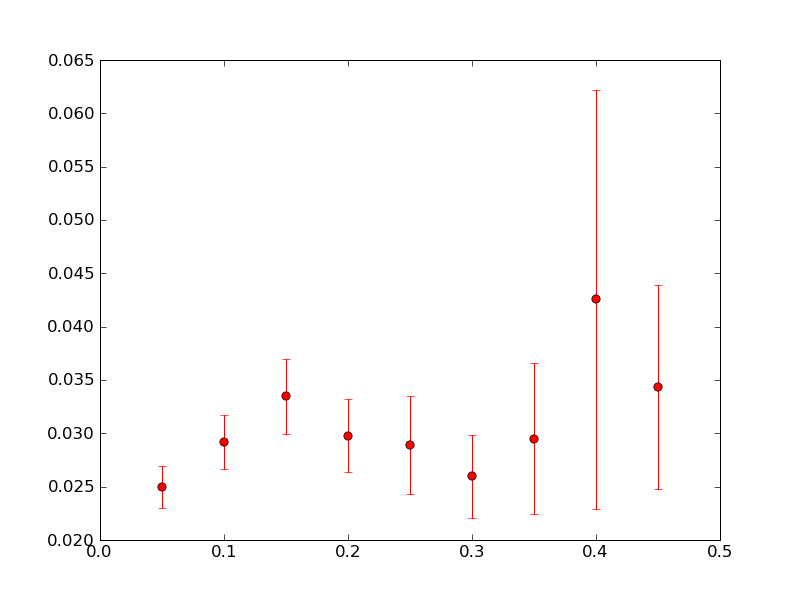
\includegraphics[width=8cm]{../figures/sixth.png}
    \caption{Community growth rates vs. ratio of closed to open triads: $6^{\rm th}$ snapshot}\label{fig:edge-f}
    \end{center}
\end{figure}

In Backstrom et al. paper \cite{group_formation}, the authors observe that if a community is highly connected, then it is less probable to grow.  This result is in contrast to the empirical evidence \cite{group_formation}  that suggests that a person is more probable to join a community,  if his/her friends inside the community are more interconnected.



In Figures \ref{fig:edge-a}-\ref{fig:edge-f}, for each snapshot, we plot the community growth rates  as a function of their clustering coefficient.  Communities are binned together with respect to clustering coefficient. The growth rate is  decreasing for the communities that have clustering coefficients  higher than $0.3$, especially for the first two snapshots.  On the other hand, the number of communities  with large clustering coefficient  is much smaller than the ones with small clustering coefficient.



In order to understand the relationship between  the clustering coefficient and the growth of a community, we divided 
the communities into two groups: $\mathcal{C}_h$ and $\mathcal{C}_l$, i.e., those that have  a clustering coefficient higher than the average, and those that have a  clustering coefficient less than the average. 



For each community $\Cc$, we computed the percentage of people in the fringe that only have one friend inside the community, i.e., 
\[
\frac{|\{x\in\mathcal{F} : \; x \textmd{ has only one friend in } \mathcal{C} \}|}{|\mathcal{F}|},
\]
and took the average among $\mathcal{C}_l$ and $\mathcal{C}_h$ separately. 
We found that for communities in $\mathcal{C}_l$ the average of this ratio is $86.6\%$, while for $\mathcal{C}_h$ it is
$76.9\%$.
Thus in the fringe of highly connected communities, on average, there are fewer people that have only one friend inside the community. Then we computed the probability 
of joining a community from its fringe for those who have only one friend inside. We took the average over $\mathcal{C}_l$ and $\mathcal{C}_h$ separately. 
The average probability of joining for such users among $\mathcal{C}_h$ communities turned out to be $8.4\times10^{-5}$, while the average of the same 
quantity for communities in $\mathcal{C}_l$ was $15.8\times 10^{-5}$ which is about twice as high. Therefore, since the majority of fringe consists of those who have only one friend inside, this partly describes the dichotomy. In other words the growth behavior  of a community is mainly determined by those in the fringe that have only one friend inside, because they are the majority of the fringe members; On the other hand, our empirical results suggest that these people are less probable to join a community if its is highly connected. 





%\newpage
%\subsection{Simulation}
%
%In this section we propose a simple model for simulating the evolution of communities through time. First we observe the evolution of a community during some initial time period, and label its members as attractive and unattractive. Then to each member of the fringe we assign a probability $p_j$, the probability of joining the community, as follows
%\[
%p_{j} = \frac{1+C_{\rm a}N_a+C_{\rm una}N_{\rm una}}{1+C_0+C_{\rm a}N_a+C_{\rm una}N_{\rm una}},
%\]
%where $N_a$ is number of attractive friends of this member inside the community, and $N_{\rm una}$ is its number of unattractive friends. Also $C_0$, $C_{\rm at}$, and $C_{\rm una}$ are constants. In our simulations, after trying to find the parameters that fit the data, we used $C_0 = 250$, $C_{\rm a} = 2$, and $C_{\rm una}=1$, which seemed to give the best results. Although the model can predict all the
%non-growing communities correctly, it could predict only about half of the growing communities as growing. We would like to try different models in order to predict the growth.
%
\subsubsection{Further study on attractiveness}

In this section we focus more on the attractiveness measure, and try to better understand its meaning and its connection to the growth of a community. For achieving this goal we pose a couple of questions, and try to answer them based on our collected data.

\begin{itemize}
\item Are recent members of a community more probable to be attractive?
\end{itemize}

It is reasonable to imagine that a person who has recently joined a community, is more likely to encourage her friends to follow her and join the community.  In Table \ref{table:rec}, for each snapshot, the average over the communities of the percentage of  attractive people in the current snapshot from those who have joined the community in the previous snapshot is shown. The table suggests that the new members are more likely to be attractive. More specifically, for the first 3 snapshots, where the time span between the snapshots is about a week, almost half of the recent members of the community are attractive. Note that the percentage of attractive people among a community is usually very small.

\begin{table}[htdp]
\caption{Average percentage of attractive people among the people who have  joined it between the current and previous snapshots}
\begin{center}
\begin{tabular}{|c|c|c|c|c|c}
\hline
snapshot & 2 & 3 & 4 & 5 \\ \hline
average percentage of   & 52.4 & 51.0 & 55.0 & 38.2 \\
attractive people  &  &  & &  \\ \hline
\end{tabular}
\end{center}
\label{table:rec}
\end{table}

%\begin{figure}
%\begin{center}
%\includegraphics[width=120mm]{../figures/rec_att.pdf}\caption{Distribution of attractivity of new comers}\label%{fig:rec_att}
%\end{center}
%\end{figure}

\begin{itemize}
\item Are there people who are always attractive?
\end{itemize}

Among the first four snapshots, for each person in a community, we computed the number of snapshots
he/she has reamined attractive. Table  \ref{table:all} shows the number of people that were attractive in just one snapshot, two snapshots etc. From the table, it seems that most people do not stay attractive for a long period of time.

\begin{table}[htdp]
\caption{Frequency of being  attractive for difference people who have been attractive at least at one snapshot}
\begin{center}
\begin{tabular}{|c|c|c|c|c|}
\hline
number of snapshots & 1 & 2 & 3 & 4  \\ \hline
number of people  & 29,255 & 6,171 & 3,954 & 34 \\ \hline
\end{tabular}
\end{center}
\label{table:all}
\end{table}%

\begin{itemize}
\item Is attractiveness of a person group-dependent?
\end{itemize}

One question to ask is whether knowing that $v\in\Vc$ is considered as attractive in  group $\Cc$ increases the chance of $v$ being attractive in some other group $\Cc'$ that contains $v$ too.  Similarly, does being unattractive in one community makes it more probable to be labeled unattractive in other groups too? In other words, are  the labels assigned to members consistent among communities or are they group-dependent? Let a person $v\in\Vc$ belong to $n_v$ different communities, $\mathcal{C}_1,\ldots,\mathcal{C}_{n_v}$. The vector  $(a_v(\Cc_1),\ldots,a_v(\Cc_{n_v})$ represents attractiveness of $v$ in these communities. For each person $v\in\Vc$, we define 
\begin{align}
p_v\triangleq\max\left(\frac{\sum\limits_{i=1}^{n_v} a_v(\Cc_i)}{n_v},1-\frac{\sum\limits_{i=1}^{n_v} a_v(\Cc_i)}{n_v}\right),
\end{align}
as a measure for the consistency of the labels assigned to people. If $v$ belongs to 5 communities and its attractiveness status vector is $(0,1,1,0,1)$  or $(1,0,0,1,0)$ in both cases $p_v=60\%$. From our data, we calculated the average of $\{p_v\}_{v\in\Vc}$ for those who are members of at least two communities.  The results for different snapshots are shown in Table \ref{table:glob} which suggests that attractiveness of a person is not a group-dependent parameter. 

\begin{table}[htdp]
\caption{Consistancy of people's attractiveness status in different communities}
\begin{center}
\begin{tabular}{|c|c|c|c|c|}\hline
snapshot & 1 & 2 & 3 & 4  \\ \hline
ratio  & 0.916 & 0.925 & 0.989 & 0.89 \\ \hline
\end{tabular}
\end{center}
\label{table:glob}
\end{table}%



